\documentclass[a4paper, twoside, titlepage]{article}

\def\ssver{1.0.0}

% ====   Packages   ====
\usepackage[left=1cm, right=1cm, top=1cm, bottom=2cm]{geometry}
\usepackage[hyperindex]{hyperref}
\usepackage{makeidx}
\usepackage{pdfpages}
\usepackage{fancyhdr}
\usepackage{graphicx}
\usepackage{adjustbox}
\usepackage{multicol}
\usepackage{totcount}
\usepackage{xcolor}

% ====   Index   ====
\makeindex

% ====   Counters   ====
\newtotcounter{songcount}
\newtotcounter{psalmcount}
\definecolor{title dark}{HTML}{7E73A7}

% ====   Footer   ====
\pagestyle{fancy}
\fancyhf{}
\cfoot{{\small\thepage} \\ v{\ssver}}
\renewcommand{\headrulewidth}{0pt}

\makeatletter

% ====   Verse   ====
\renewcommand{\verse}{\@versei}
\newcommand{\@versei}{\@ifnextchar\end{\@verseend}{\@verseii}} % chktex 10
\newcommand{\@verseii}[1]{#1\par\@versei}
\newcommand{\@verseend}[1]{\vskip1em}

% ====   Chorus   ====
\newcommand{\chorus}{\@chorusi}
\newcommand{\@chorusi}{\@ifnextchar\end{\@chorusend}{\@chorusii}} % chktex 10
\newcommand{\@chorusii}[1]{\quad\textit{#1}\par\@chorusi}
\newcommand{\@chorusend}[1]{\vskip1em}

% ====   Bridge   ====
\newcommand{\bridge}{\@bridgei}
\newcommand{\@bridgei}{\@ifnextchar\end{\@bridgeend}{\@bridgeii}} % chktex 10
\newcommand{\@bridgeii}[1]{\textit{#1}\par\@bridgei}
\newcommand{\@bridgeend}[1]{\vskip1em}

\makeatother

% ====   Song   ====
\newenvironment{song}[1]%
{%
    \begin{minipage}[t]{0.94\columnwidth}{\stepcounter{songcount}\textbf{\large #1}\index{#1}}%
        \par\vspace{2pt}
}%
{%
    \end{minipage}%
    \vspace{2em}%
}

% ====   Psalm   ====
\newenvironment{psalm}[2]%
{%
    \begin{minipage}[t]{0.94\columnwidth}%
        \begin{center}{\stepcounter{psalmcount}\textbf{\large #1}\index{#1}{\normalsize #2}}%
            \par\vspace{2pt}
}%
{%
        \end{center}%
    \end{minipage}%
    \vspace{2em}%
}%

% ====   Utitilty Commands   ====
\newcommand{\extra}[1]{\textit{\normalsize (#1)}}
\renewcommand{\sp}{\textit{\normalsize (Sing Psalms)}}
\newcommand{\tr}{\textit{\normalsize (Scottish Psalter)}}
\newcommand{\LORD}{\textsc{Lord}}
\newcommand{\cp}[1]{{\tiny\ttfamily#1}}

% ====   Document   ====
\begin{document}
\sffamily

\begin{titlepage}
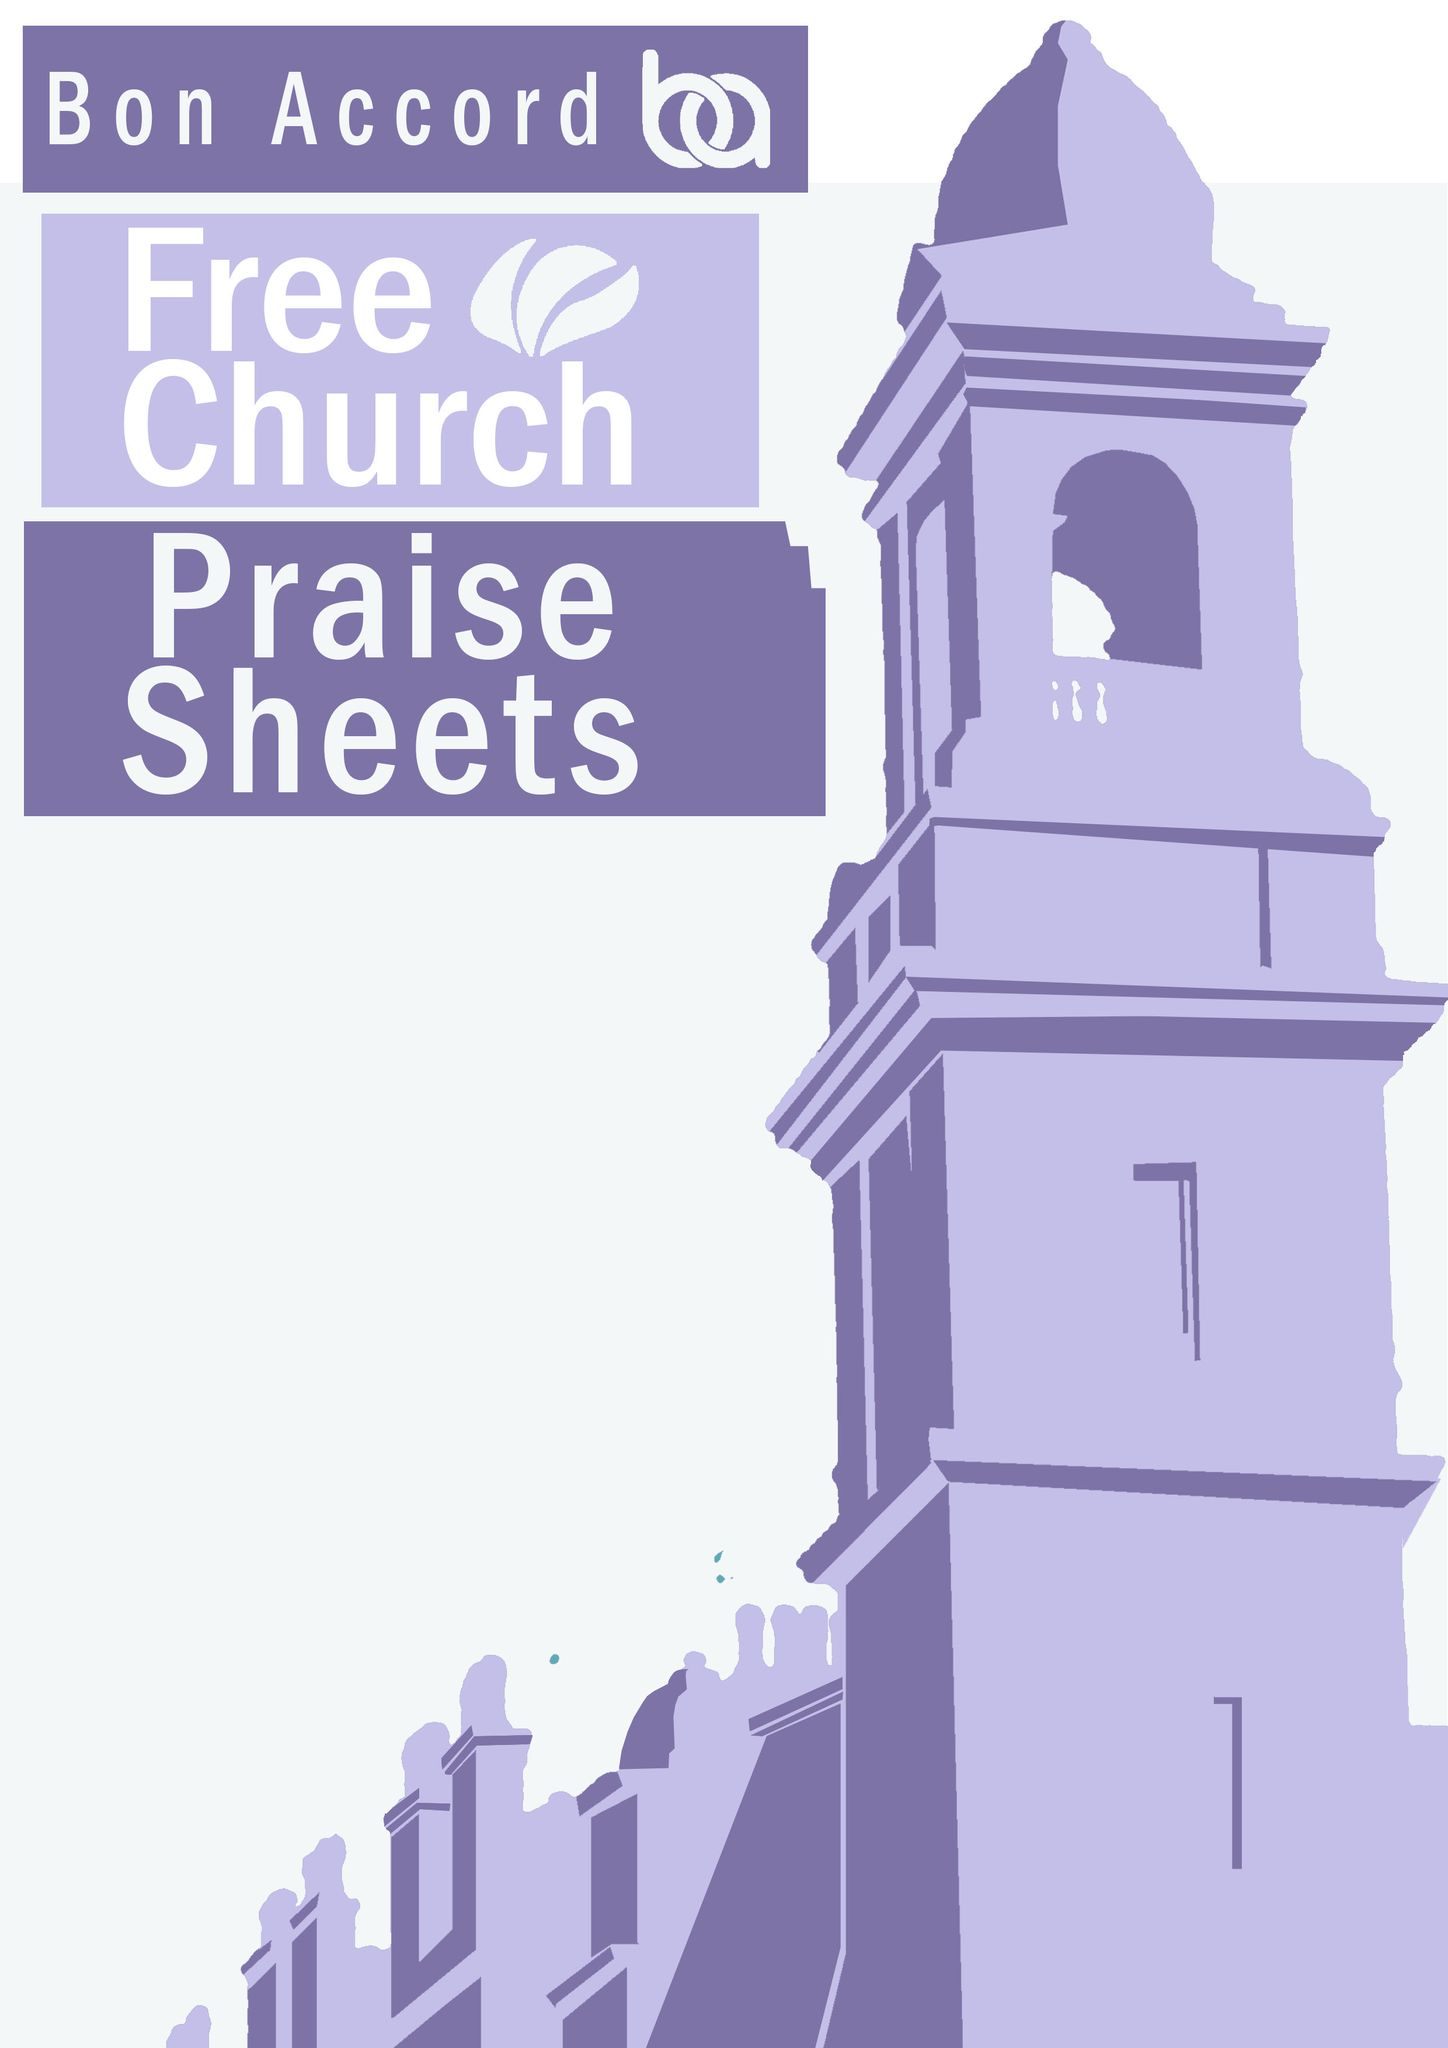
\includepdf{./titleimage.jpg}
\end{titlepage}

\setcounter{page}{2}  % Make title page, page 1
\printindex
\begin{multicols}{2}
\raggedcolumns{}

% ====   As The Deer Pants   ====
\begin{song}{As The Deer Pants}
    \verse
    {As the deer pants for the water}
    {So my soul longs after Thee.}
    {You alone are my heart's desire}
    {And I long to worship You}
    \end
    \chorus
    {You alone are my Strength, my Shield}
    {To You alone may my spirit yield}
    {You alone are my heart's desire}
    {And I long to worship Thee}
    \end
    \verse
    {You're my friend and You are my brother,}
    {Even though you are a king.}
    {I love You more than any other,}
    {So much more than anything.}
    \end
    \verse
    {I want You more than gold or silver,}
    {Only You can satisfy.}
    {You alone are the real joy Giver,}
    {And the Apple of my eye.}
    \end
\end{song}

% ====   Because He Lives   ====
\begin{song}{Because He Lives}
    \verse
    {God sent His Son, they called him Jesus}
    {He came to love, heal and forgive}
    {He bled and died to buy my pardon}
    {An empty grave is there to prove my Saviour lives}
    \end
    \chorus
    {Because He lives, I can face tomorrow}
    {Because He lives all fear is gone}
    {Because I know He holds the future}
    {My life is worth the living just because He lives}
    \end
    \verse
    {How sweet to hold a new born baby}
    {And feel the pride and joy He gives}
    {But better still, the calm assurance}
    {That child can face uncertain days because He lives}
    \end
    \verse
    {And then one day I'll cross the river}
    {I'll fight life's final war with pain}
    {And then as death gives way to victory}
    {I'll see the lights of glory and I'll know He lives}
    \end
\end{song}

\end{multicols}
\end{document}
